\chapter{\hspace*{3pt} The Wikipedia Category Graph}
\label{chapter:graph}

Exploiting the underlying structure of Wikipedia requires a way of representing it.  In this chapter, a topological analysis of this structure represented as a directed graph has been performed.

The primary goal of the analysis expressed in this chapter is understanding the organization of the Wikipedia body of knowledge regarding its structure of categories, as well as the possibilities and challenges that emerge from decoding this underlying structure. 

The inspiration for this chapter comes from the work presented by Zesch and Gurevych \cite{zesch2007analysis}, where they showed that the \gls{wcg} is a scale-free, small-world graph, similar to other semantic networks such as WordNet \cite{miller1998wordnet} or Thesaurus.com\footnote{\url{https://www.thesaurus.com/}}. They concluded that the \gls{wcg} could be used for \gls{nlp} tasks, where other semantic networks have been traditionally employed. Although their work has been useful in supporting many types of research in the past years, the analysis was restricted to the German version of Wikipedia as it stood in 2007. 

This thesis contains an up-to-date review of a more recent version of Wikipedia, to obtain insights on how the structure of the \gls{wcg} can influence the proposed method and guide the development of future work. 

\section{\hspace*{3pt} The Category Graph}


A category graph is a way of representing existing relationships between categories, such as which subcategories can be reached from one another. Figure \ref{fig:graph-example-wcg} illustrates how the categories are organized and connected if they are represented as a graph. The nodes in the graph represent categories, and the edges represent the relationships between them. 

The graph illustrated in figure \ref{fig:graph-example-wcg} is directed with each edge representing the relationship between a pair of categories (e.g., C1 1 is a subcategory of TC-1 since the arrow points from C1 to TC1). TC-1, TC-2, and TC-3 represent the top-level categories of Wikipedia. At the time of writing, there are a total of 19 top-level categories in the English Wikipedia that summarize the entirety of the body of knowledge encoded within its articles (namely Arts, Culture, Games, Geography, Health, History, Humanities, Industry, Law, Life, Mathematics, Matter, Nature, Philosophy, People, Reference Works, Religion, Science and Technology, and Society). The HC1 represents a hidden category. Hidden categories are not displayed in the Wikipedia articles to general users, even if the article is placed under that category. These categories are mainly used for internal organization and do not provide any meaning - for that reason, they have been omitted from the graph.

The details of information extraction from Wikipedia, and the ways in this information was filtered in order to assemble and represent the \gls{wcg} for carrying out the analysis (as described in this chapter) are reported in Appendix \ref{app:representing-structre}. The use of the graph as the basis for the proposed approach is also described.

\begin{figure}[H]
  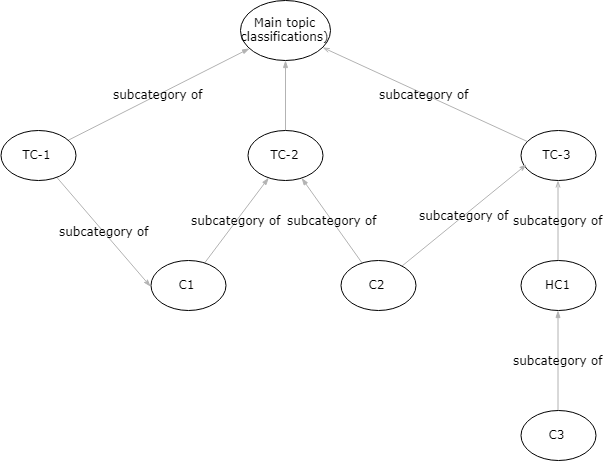
\includegraphics[width=\linewidth]{imgs/wcg-example}
  \caption{Simplified example of the underlying structure of the \gls{wcg}}
  \label{fig:graph-example-wcg}
\end{figure}



\section{\hspace*{3pt} Small-world networks (SW)}

According to Steyvers and Tenenbaum \cite{steyvers2005large}, interest in studying the small-world phenomenon originated with social network studies when the results suggested that any two people were, on average, separated by only a few
acquaintances or friends (so-called ``six degrees of separation”). While the finding of very short path lengths between random pairs of nodes in a network may seem unexpected, the phenomenon is well-described by even the simplest models of random graph theory, such as the one by Erdös and Réyni \cite{erdos1960evolution}. In an Erdös and Réyni random graph with $n$ nodes, any pair of nodes is connected by an edge with probability $p$. When $p$ is sufficiently high, the whole network becomes connected: the average path-length, $L$, grows logarithmically with $n$, the size of the network.


Watts and Strogatz \cite{watts1998collective} formally defined small-world networks as a class of networks that are highly clustered, like regular networks, yet have small characteristic path lengths, like random graphs. These characteristics result in networks with unique properties of regional specialization with efficient information transfer. 

Most real-world networks, such as the \gls{www}, networks of scientific collaborators, and metabolic networks in biology do not have the homogeneous distribution of degree (the degree of a node is the number of neighbors a node has) that regular or random networks have. The number of connections each node has varies considerably in most networks, and they are positioned somewhere between regular and random networks. \cite{steyvers2005large}

Figure \ref{fig:taxonomy-networks} displays the difference between distribution of nodes in a regular network (\ref{fig:network-taxonomy}, a small-world network (\ref{fig:network-smallworld}) and a random network (\ref{fig:network-random}). 


\begin{figure}[!htb]
\minipage{0.32\textwidth}
  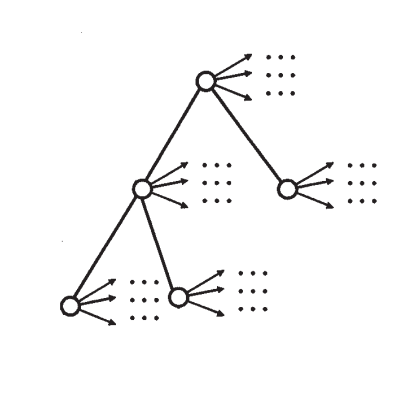
\includegraphics[width=\linewidth]{taxonomy}
  \caption{A tree-structured hierarchy}\label{fig:network-taxonomy}
\endminipage\hfill
\minipage{0.32\textwidth}
  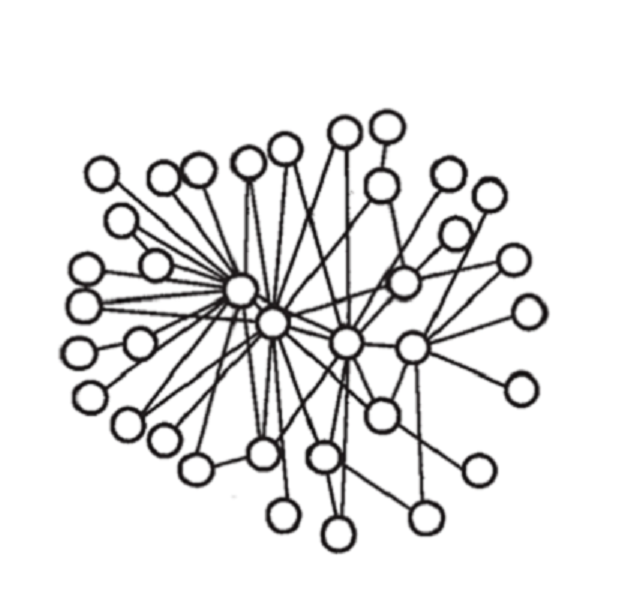
\includegraphics[width=\linewidth]{sfsw}
  \caption{Scale-free small-world graph}\label{fig:network-smallworld}
\endminipage\hfill
\minipage{0.32\textwidth}%
  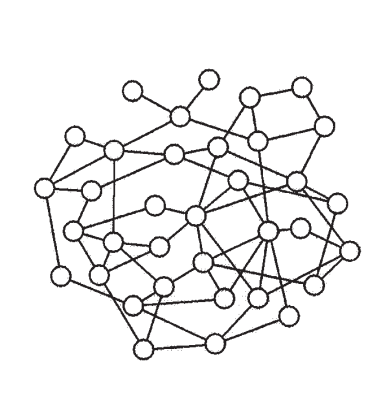
\includegraphics[width=\linewidth]{random}
  \caption{An arbitrary, unstructured random graph}\label{fig:network-random}
\endminipage
\caption{Structures of semantic networks adapted from Steyvers and Tenenbaum \cite{steyvers2005large}}
\label{fig:taxonomy-networks}
\end{figure}


Steyvers and Tenenbaum \cite{steyvers2005large}, analyzed different large-scale semantic networks (such as WordNet \cite{miller1998wordnet} and Thesaurus.com) regarding Sparsity, Connectedness, Path-Lengths, Clustering coefficient and degree distribution, concluding that all of them exhibit a scale-free pattern. These metrics are described and analyzed in the context of the \gls{wcg} below.




\subsection{\hspace*{3pt} Sparsity and Connectedness}

The \gls{wcg} assembled for the experiments contains $1,475,806$ nodes and $4,091,417$ edges. Each node
represents a category and each edge represents a relationship of the type ``Subcategory Of". 

The density $D$ of a graph $G$ is the ratio of edges in $G$ to the maximum possible number of edges, defined in a directed graph as  
\begin{equation}
D={\frac  {|E|}{|V|\,(|V|-1)}}
\end{equation} where $V$ is the set of nodes and $E$ is the set of edges.

A graph is said to be dense when the number of existing edges is close to the number of possible edges. In the \gls{wcg}, the density is $1.878519 * 10^{-6}$. As in the semantic structures analyzed in \cite{steyvers2005large}, on average, a node is connected to only a tiny percentage of other nodes. 

In the \gls{wcg} examined for this thesis, the largest connected component contained 99.23\% of the total nodes.
Despite the sparsity, networks that are not random form one large connected component: from one node, any other node can be reached by some associative path. 
%But 99% is very dense? Dense = opposite of sparsity



\subsection{\hspace*{3pt} Path lengths}

A path in a graph is a sequence of alternating nodes and edges that starts with a node and ends with another node in such a way that adjacent nodes and edges in the sequence are incidental to each other \cite{newman2010networks}. Nodes or edges can appear in the same path multiple times, and the number of edges in a path is the length of that given path. If a graph is connected, then any node can be reached via a finite-length path starting from any other node. The shortest path between a pair of nodes is called a geodesic path, and there can be more than one such path.

The average path length, a concept in the field of network topology, is defined as the average number of steps in the shortest paths for all possible pairs of nodes in the graph. In directed graphs, the average path length is calculated as follows:

\begin{equation}
l_{G}={\frac  {1}{2 * n\cdot (n-1)}}\cdot \sum _{{i\neq j}}d(v_{i},v_{j})
\end{equation}

where $d(v_{i},v_{j})$ denotes the shortest distance between $v_i$ and $v_j$ and $n$ is the number of nodes in the graph $G$. 

If two nodes are disconnected (i.e., no path exists between them), the path length between these nodes is infinite. Consequently, if a graph contains disconnected components, the average shortest path length $l_G$ tends to infinity. 
Given that the \gls{wcg} is not completely connected, to avoid infinity, the average shortest path length was calculated for the largest connected component. As a result, the $l_G$ is $20,9343$. The shortest path length distribution is displayed in figure \ref{fig:path-distribution} where the y-axis represents the number of nodes and the x-axis represents the number average path length. 


\begin{figure}[H]
  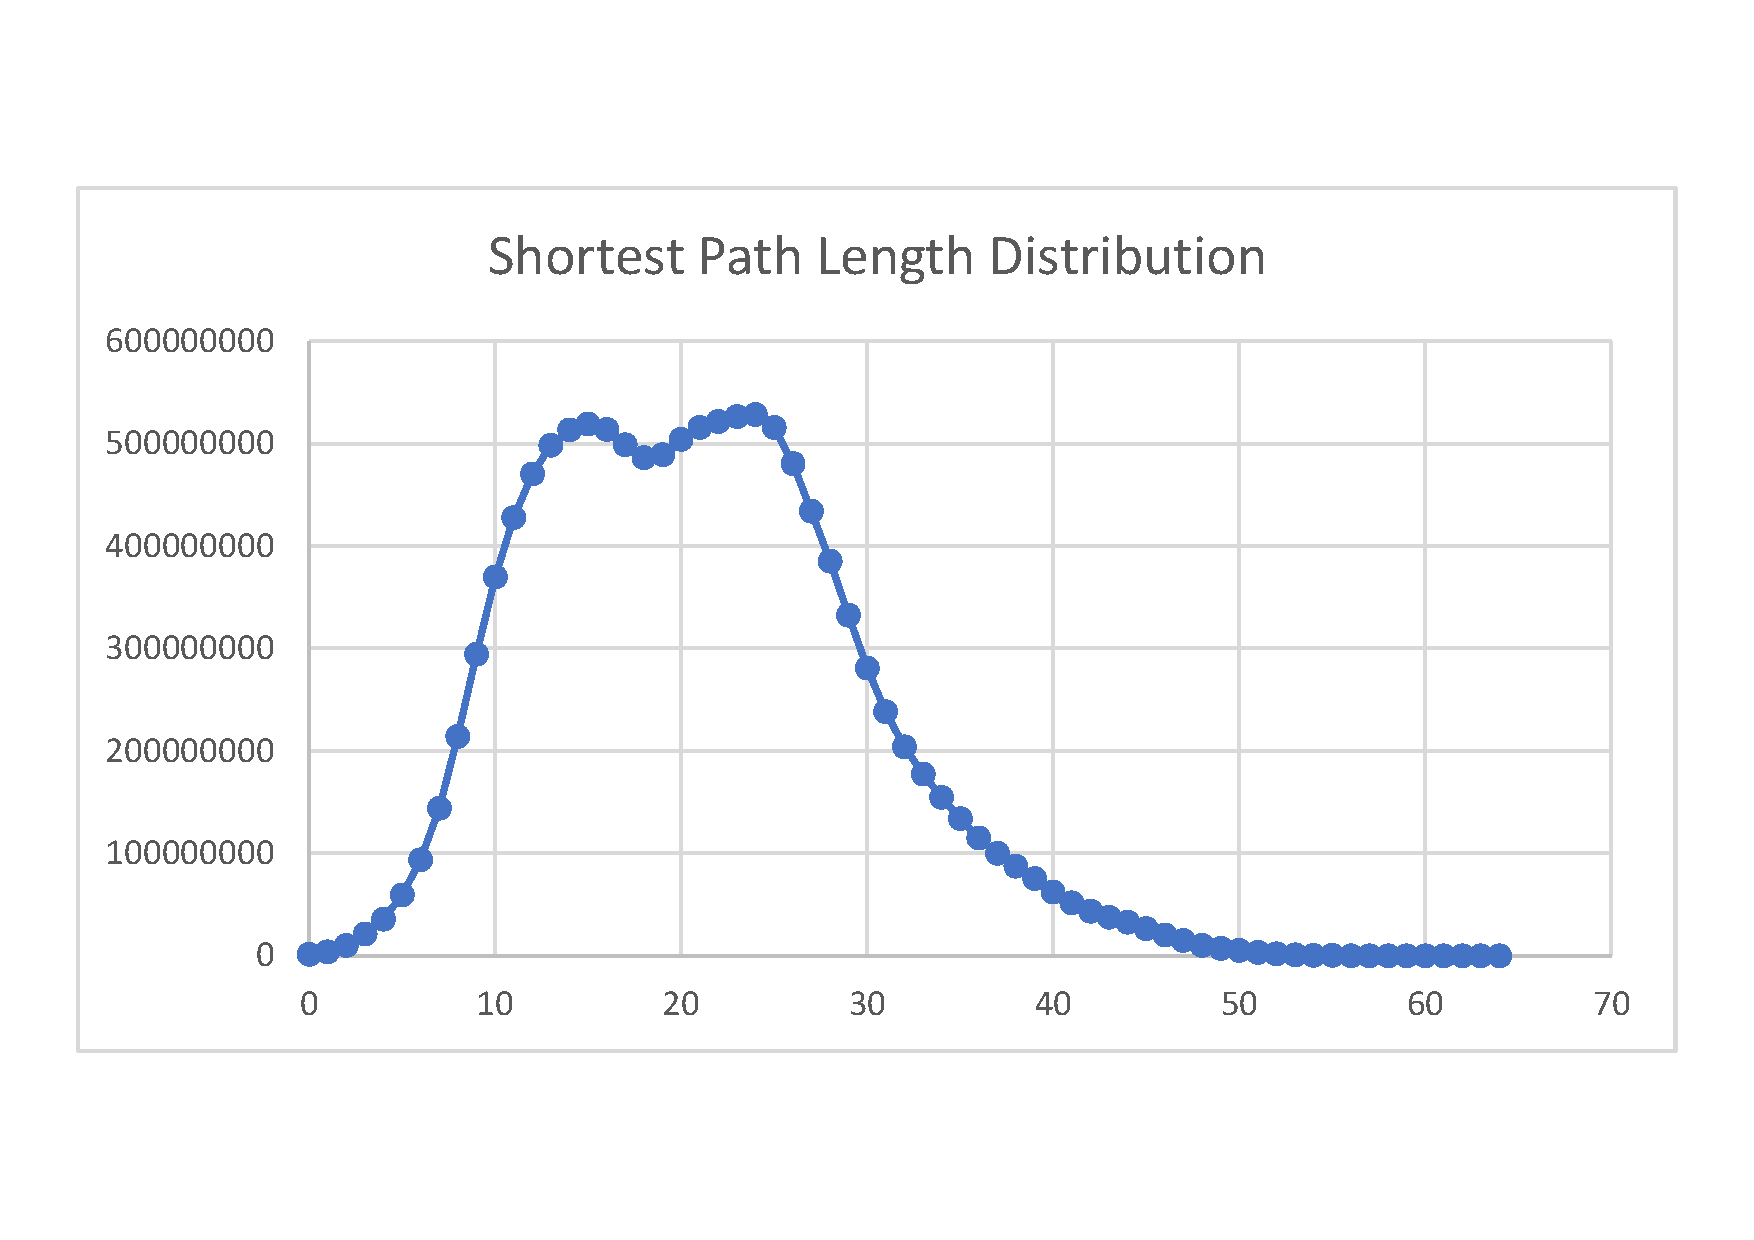
\includegraphics[width=\linewidth]{path_frequency2}
  \caption{Shortest path length distribution on the \gls{wcg}}
  \label{fig:path-distribution}
\end{figure}


\subsection{\hspace*{3pt} Clustering Coefficient}


Another important metric for understanding the topology of a graph is its clustering coefficient. The clustering coefficient of a node represents the probability that if two of its neighbors are randomly chosen, they will also be connected by an edge. More precisely, if a node has $t$ neighbors, then there are $t(t-1)/2$ possible edges that connect those neighbors. 
The local clustering coefficient for a node is then given by the proportion of edges between nodes within its neighborhood divided by the number of links that could exist between them. 

The clustering coefficient $C$ of the whole graph $G$ is the average of the local clustering coefficients $C(v)$ of all nodes $v \in V$. 

Figure \ref{fig:clustering-example} illustrates how the clustering coefficient of a node is calculated.

\begin{figure}[H]
  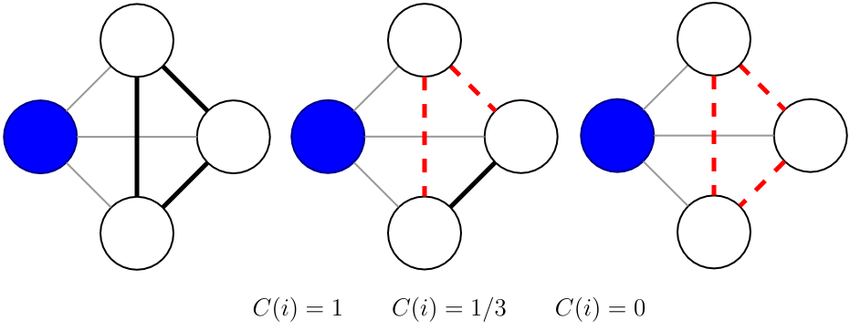
\includegraphics[width=\linewidth]{imgs/clustering}
  \caption{Example of how the clustering coefficient of a node is calculated based on the probability of the neighbors of the node $i$ are also neighbors among themselves}
  \label{fig:clustering-example}
\end{figure}

The \gls{wcg} has a clustering coefficient of $0.0461$.  This value of clustering is orders of magnitude larger than can be expected from random graphs of equivalent size and density. The same phenomenon was observed in the networks analyzed in \cite{steyvers2005large}. The impact of clustering in scale-free networks is described below.



\subsection{\hspace*{3pt} Degree Distribution}


The indegree of node $v$ is the total number of connections into node $v$; the outdegree of node $v$ is the total number of connections coming out from the node. The indegree and outdegree of the graph is the average of the degree of each node presented in the graph.

Large graphs such as the \gls{wcg} are complex structures, as the connections among the nodes can present complicated patterns. 
While studying complex networks, it is common to develop simplified measures that capture some elements of the structure. The degree distribution of a complex network is often described in this context. 

The degree distribution of a graph is the probability distribution that a randomly chosen node will have a degree $k$. In directed graphs the degree distribution is a two-dimensional distribution, so that $P_{\text{deg}}(k^{\text{in}},k^{\text{out}} ) =$ the portion of nodes in the graph with indegree $k^{\text{in}}$ and outdegree $k^{\text{out}}$.


There is a large class of so-called scale-free networks, characterized by a highly heterogeneous degree distribution, which follows a power-law\footnote{A relationship between two variables such that one is proportional to a fixed power of the other.}. They are called scale-free because zooming in on any part of the distribution does not change the shape of the network: there is a few, but a significant number of nodes with many connections and there is a trailing tail of nodes with a very few links at each level of magnification \cite{steyvers2005large}.


A %remarkable peculiarity 
characteristic of a scale-free network, derived from its degree distribution, is its tolerance to mistakes. If a random node is disconnected from the network, the highest probability is that this node has a low degree, causing a little impact for the interconnectivity of the remaining network.


Small-world networks tend to show a power-law distribution which means that the fraction $P(k)$ of nodes in the graph having $k$ connections to other nodes varies as a power of some attribute $\alpha$, as in: 
\begin{equation}
P(k)=Ck^{-\alpha}
\end{equation}


To define the best with the best fitting power-law curves, the method applied is defined in \cite{clauset2009power} as \begin{equation}
\alpha = 1 +n\left[\sum_{i=1}^n\ln\frac{x_i}{x_{\min}}\right]^{-1}
\end{equation}
where $x_{\min}$ is a lower cutoff, below which the power-law cannot be observed. The parameters observed are shown in table \ref{tab:power-law-params}.

\begin{table}[ht!]
\centering
\begin{tabular}{@{}lll@{}}
\toprule
           & $\alpha$ & $x\_{min}$ \\ \midrule
indegree  & 2,4124 & 10         \\
outdegree & 4,5603 & 12         \\ \bottomrule
\end{tabular}
\caption{Power-law parameters of the \gls{wcg}}
\label{tab:power-law-params}
\end{table}


Figure \ref{fig:in-and-out-degree} shows the degree distribution for the \gls{wcg} in log-log\footnote{
A two-dimensional graph of numerical data that uses logarithmic scales on both the horizontal and vertical axes. 
} plot. The $x$-axis shows the degree while the $y$-axis shows the count of nodes with such degree. 

\begin{figure}[!h]
\centering
\begin{subfigure}{0.49\textwidth}
\centering
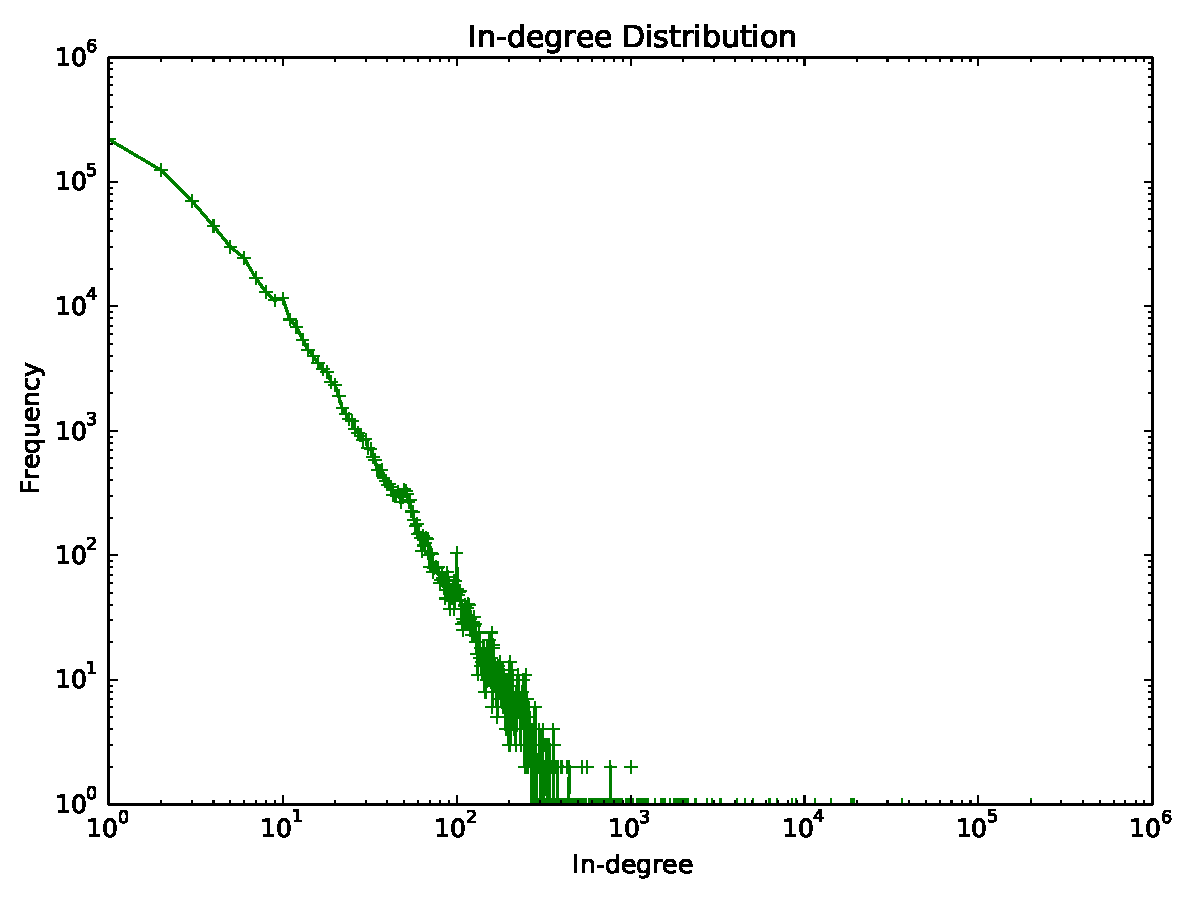
\includegraphics[width = \textwidth]{wikipedia-in-deg-dist.pdf}
\caption{Distribution of indegree}
\label{fig:left}
\end{subfigure}
\begin{subfigure}{0.49\textwidth}
\centering
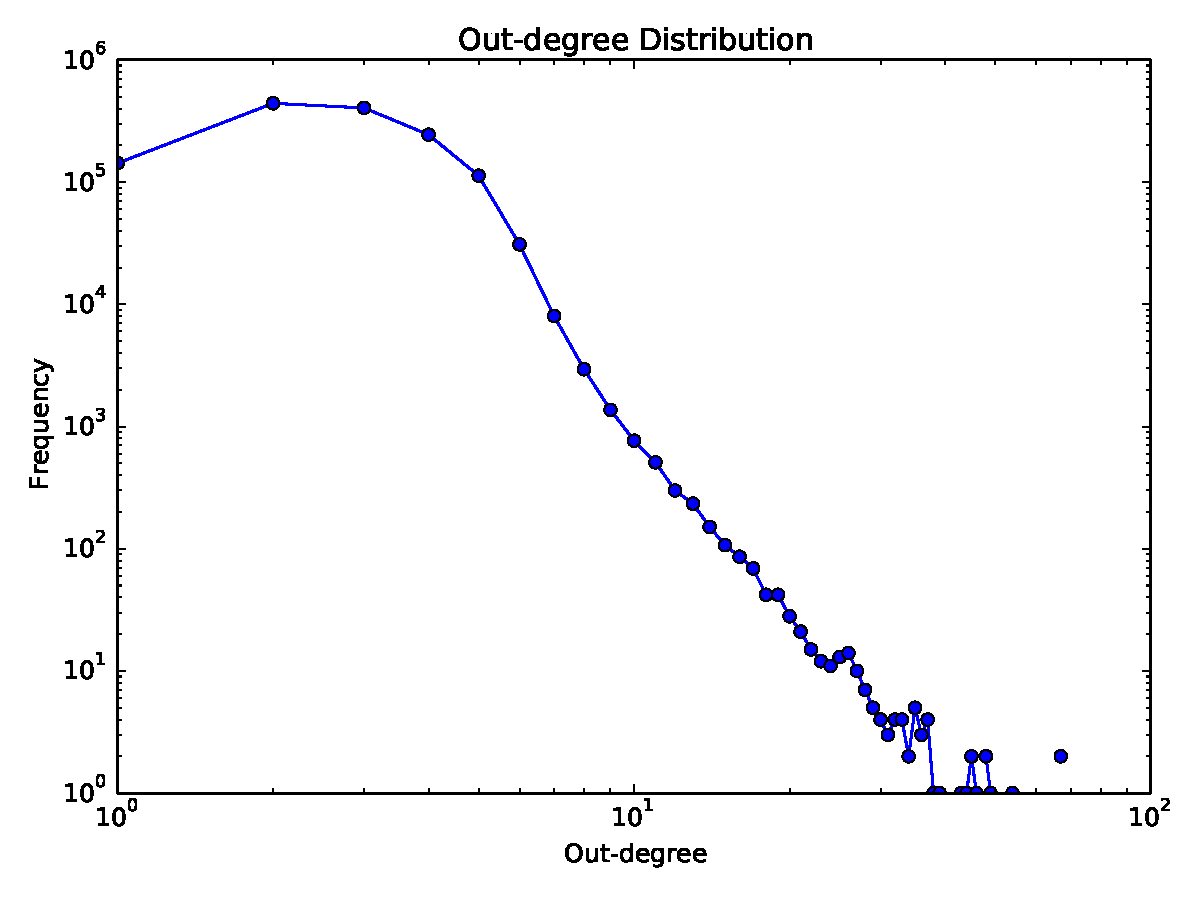
\includegraphics[width = \textwidth]{wikipedia-out-deg-dist.pdf}
\caption{Distribution of outdegree}
\label{fig:right}
\end{subfigure}
\caption{Indegree and outdegree distributions}
\label{fig:in-and-out-degree}
\end{figure}


Based on the analysis of the \gls{wcg} degree distribution, as presented by the plot in figure \ref{fig:in-and-out-degree} and the exponent displayed in table \ref{tab:power-law-params}, it is demonstrated that the \gls{wcg} nodes follow a power-law distribution. Hence it can be consider as a scale-free network. The same was reported in \cite{steyvers2005large} regarding other large semantic networks. 


\subsection{\hspace*{3pt} Empirical demonstration of small-worldness}

Based on the metrics evaluated by Steyvers and Tenenbaum \cite {steyvers2005large} and reported in this chapter, it is possible to infer that the structure of the \gls{wcg} is very similar to the  small-world networks. However, to support this statement, it is demonstrated based on a mathematical method below.  

Humphries and Gurney \cite{humphries2008network} described a mathematical method to determine whether or not a graph can be considered a small-world based on the comparison of the graph parameters (\gls {wcg}) with a random graph with the same proportions.

Formally, a graph $G$ with $n$ nodes and $m$ edges is said to be a small-world if it has a similar path length but greater clustering of nodes than an equivalent Erdös-Rényi (E–R) random graph with the same $m$ and $n$. Let $L_g$ be the mean shortest path length of $G$ and $C_g$ its clustering coefficient. Let $L_{rand}$ and  $C_{rand}$ be the corresponding quantities for the corresponding E–R random graph. According to the empirical experiments performed in \cite{humphries2008network}, a graph $G$ is said to be a small-world network if $L_g \ge L_{rand}$ and $ C_g \gg C_{rand}$. Table \ref{small-worldness} shows the summarized values for the \gls{wcg} at the centre of this thesis, and for a random graph with the same number of nodes and edges. 


\begin{table}[!h]
\centering
\caption{Empirical demonstration of small-worldness of the \gls{wcg}. }
\begin{tabular}{@{}lllll@{}}
\toprule
    & $L_g$       & $L_{rand}$       & $C_{g}$           & $C_{rand}$        \\ \midrule
\gls{wcg} & 20.9343 & 19.5389 & 0.0461 & 0.00000003 \\ \bottomrule
\end{tabular}

\label{small-worldness}
\end{table}

The \gls{wcg} exhibits small-world behavior, with an average shortest path length close to that of a random network of the same size. The clustering coefficient, however, is orders of magnitude higher than in the random graph.  


\section{\hspace*{3pt} Final Consideration}

In this chapter, the representation of the categories of Wikipedia and the relationships between them in the form of a directed graph has been described. An analysis of the topology of the graph was performed, empirically demonstrating that, as with other large-scale semantic networks, the \gls{wcg} can also be characterized as a small-world and scale-free network.

Challenges encountered in this analysis included the considerable computational power required by the processes of both the information extraction and the analysis. This is likely to be the main reason why most of the existing literature on the topic has tended to focus on the analysis of semantic networks that are much smaller, but also quickly out of date.

This analysis supports some critical decisions related to the proposed method. The aggregation of categories consists of navigating the Category Graph from each category extracted from the named entities in the text towards the top-level categories. 
Considering that the \gls{wcg} is a small world, navigating towards all paths would be nonsensical, since each category can be reached from any other. However, because the \gls{wcg} resembles other semantic networks commonly used in \gls{nlp} and \gls{ir}  applications, the shortest paths can be used,  as in this type of graph they carry a robust semantic relation \cite{mihalcea2011graph}.

As a scale-free network, the structure of the the \gls{wcg} is notably fault tolerant. The categorization process in Wikipedia is a continuous work-in-progress, as users edit, remove, and add categories frequently. However, the probability that an edit spoils the overall structure of the graph is very low since most categories do not have a high degree of connection to the whole graph.

In addition to the fact that it is scale-free, \gls {wcg} has another significant advantage for categorization: the subjects are divided into well-connected neighborhoods, and the neighborhoods are interconnected to some extent. In practice, this means that specific knowledge about a subject is presented in a well-connected way, while transversal knowledge can also be captured from this structure.